\section{Evaluation}
This section describes the in-depth analysis of 16 micro-benchmark experiments.
The experiments are partitioned into for sections; single core/multi-core and TCP/UDP.
On single core we evaluate TX/RX and RR on multi-core we evaluate TX/RX and Bi-Directional traffic.

\subsection{Summery of Results}
Tables ~\ref{tab:exec-single} and summersize the micro-benchmark results and analysis.
\begin{table*}
\centering
\begin{tabular}{l|c|c|c}
Experiment & vanilla & \oursys & reason\\\hline
Single UDP TX (Gb/s)& 44 & 52 (+18\%) &  instructions per packet\\
Single UDP RX & 90 & 52 & Faulty experiment\\
Single UDP RR (60B pps)& 186k & 195k(+4.8\%) & see discussion\\\hline
Single TCP TX (Gb/s)& 60.33 & 62.45 (+3.5\%) & Need manual inspection\\
Single TCP RX (Gb/s)& 55.3 & 56.48 (+2.7\%)& slightly better IPC\\
Single TCP RR (pps)& 176.6 & 185.2 (+5.1\%)& instructions per packet\\\hline
\end{tabular}
\caption{\label{tab:exec-single}Single core results breakdown.}
\end{table*}
\begin{table*}
\centering
\begin{tabular}{l|c|c|c}
Experiment & vanilla & \oursys & reason\\\hline
Multi UDP TX (Gb/s|CPU)& 147 | 100\% & 200 | 50\% &  Locking issues in vanilla\\
Multi UDP RX (Gb/s|CPU)& 200 | 40\%  & 200 | 40\% & Equal results\\
Multi UDP BI (Gb/s|CPU)& 240 | 100\% & 360 | 88\% &Locking in vanilla, \oursys limited by mem BW\\\hline
Multi TCP TX (Gb/s)& 187.41|39.7\% & 187.7|37.37\% & (+6.4\%)better instructions per packet - (alloc\_skb)\\
Multi TCP RX (Gb/s)& 200|46\% & 200|46\%& Equal results\\
Multi TCP BI (pps)& 350|64.13\% & 350|61.29\%& Not clear why 400Gb/s not reached\\\hline
\end{tabular}
\caption{\label{tab:exec-multi}Multi-core results breakdown.}
\end{table*}

\subsection{Single-core UDP}
All single core tests are aimed to utilize 100\% of the CPU. In UDP-TX we have a single netperf flow sending 63KB datagrams. Using a dedicated memory allocator, boosts performance by 17.4\% in single core UDP TX experiment.

\begin{figure}
\centering
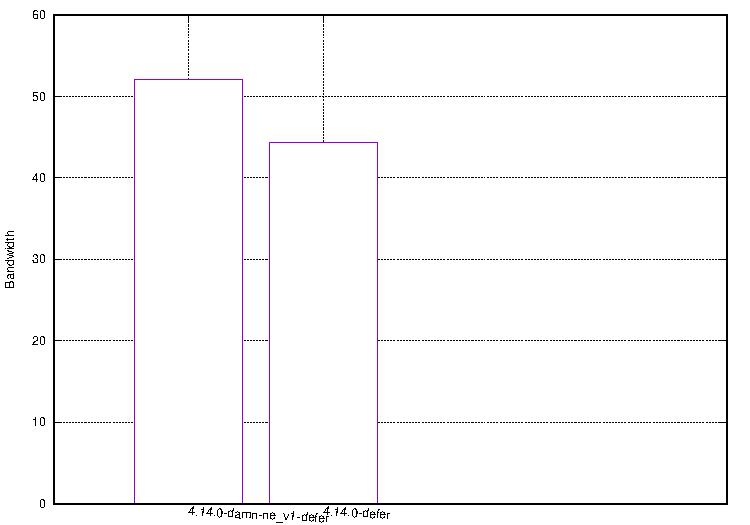
\includegraphics[width=0.5\textwidth]{figures/single_udp_tx_Bandwidth.pdf}
\caption{\label{fig:s-u-tx} Dan, I know that the text on the graph is too small. Single-core UDP TX.}
\end{figure}

\begin{figure}
\centering
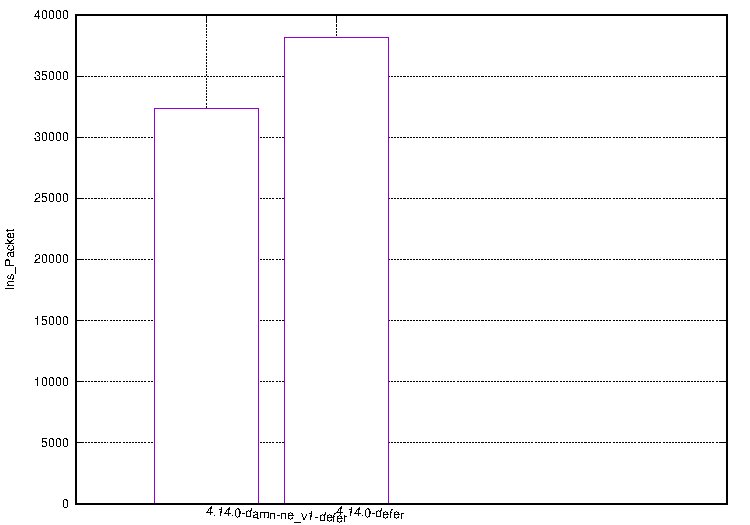
\includegraphics[width=0.5\textwidth]{figures/single_udp_tx_Ins_Packet.pdf}
\caption{\label{fig:s-u-tx-ipp} Single-core UDP TX, Instructions per packet.}
\end{figure}

In the case of single UDP TX, the main benefit is from faster allocation API. In figure \ref{fig:s-u-tx-ipp} we see the number of instructions per packet. The instructions per packet has the inverse ratio to the B/W, with 3798 vs 3235 cycles to vanilla and \oursys respectively. Curiously, both kernel versions had an almost identical number of cycles per second at 2.6e+9. In table \ref{tab:s-u-tx-funcs} we see the break down of cycles per packet. It seems that the major bulk of the 563 cycles that are saved by \oursys per packet come from the myriad of small functions removed from the allocation path. The path a pakcet takes in the vanilla kernel has 224 functions than in \oursys. 
\newline
Conclusion, although the system with \oursys seems to show better l2 and llc utilization(not seen in the above discussion).
The instructions per packet seem to provide the correct answer.

\begin{table}
\centering
\begin{tabular}{l|r|r}
Function & \oursys (3235)& vanilla (3798)\\\hline
csum\_partial\_copy\_generic & 43.85\% (1419) & 35.2\% (1337)\\
\_raw\_spinlock (\_\_dev\_queue\_xmit) & 4.75\% (153) & 4.45\% (169)\\
mlx5\_xmit & 3.43\% (111) & 2.52\% (96)\\
get\_page\_from\_free\_list & - & 2.43\% (92)\\
ip\_append\_data & 1.95\% (63) & 1.66\% (63)\\
alloc\_skb & 1.92\% (62) & 1.28\% (49)\\
ip\_finish\_output2 & 1.77\% (57) & 1.60\% (61)\\
mlx5\_poll\_tx\_cq & 1.64\% (53) & 1.40\% (53)\\
\_\_free\_pages\_ok & - & 1.37\% (52)\\
other & 59.31\% (1316) & 51.91\% (1826)
\end{tabular}
\caption{\label{tab:s-u-tx-funcs}Function breakdown.}
\end{table}

\begin{table}
\centering
\begin{tabular}{l|r|r}
Function & \oursys (3235)& vanilla (3798)\\\hline
csum\_partial\_copy\_generic & 50.09\% (1620.4) & 38.93\%(1478.6)\\
alloc\_skb & 5.66\% (183)& 8.66\% (328)\\
mlx5\_napi & 6.35\% (205)& 7.31\%(277)\\
\_raw\_spinlock (\_\_dev\_queue\_xmit) & 4.79\% (155) & 5.28\% (200)\\
skb\_free\_head & 1.07 (35)\% & 3.06\% (116)\\
other & 28.04\% (907)& 32.19\%(1222)\\
\end{tabular}
\caption{\label{tab:s-u-tx-funcs_child}Function breakdown with child.}
\end{table}
\subsection{Single UDP RR}
The answer is a balance between better IPC and higher(!) instructions per packet. The higher instructions per packet is due do higher interrupt count. Faster processing leads to NAPI failing to keep up (need coraboration, with irq count and packet/irq).  